%%% Hlavní soubor. Zde se definují základní parametry a odkazuje se na ostatní části. %%%

%% Verze pro jednostranný tisk:
% Okraje: levý 40mm, pravý 25mm, horní a dolní 25mm
% (ale pozor, LaTeX si sám přidává 1in)
\documentclass[12pt,a4paper]{report}
\setlength\textwidth{145mm}
\setlength\textheight{247mm}
\setlength\oddsidemargin{15mm}
\setlength\evensidemargin{15mm}
\setlength\topmargin{0mm}
\setlength\headsep{0mm}
\setlength\headheight{0mm}
% \openright zařídí, aby následující text začínal na pravé straně knihy
\let\openright=\clearpage

%% Pokud tiskneme oboustranně:
% \documentclass[12pt,a4paper,twoside,openright]{report}
% \setlength\textwidth{145mm}
% \setlength\textheight{247mm}
% \setlength\oddsidemargin{14.2mm}
% \setlength\evensidemargin{0mm}
% \setlength\topmargin{0mm}
% \setlength\headsep{0mm}
% \setlength\headheight{0mm}
% \let\openright=\cleardoublepage

%% Vytváříme PDF/A-2u
\usepackage[a-2u]{pdfx}

%% Přepneme na českou sazbu a fonty Libertine
\usepackage[czech]{babel}
\usepackage[T1]{fontenc}
\usepackage{libertine}
\usepackage{libertinust1math}
\usepackage{textcomp}
%\usepackage{microtype}

%% Použité kódování znaků: obvykle latin2, cp1250 nebo utf8:
\usepackage[utf8]{inputenc}

%%% Další užitečné balíčky (jsou součástí běžných distribucí LaTeXu)
\usepackage{amsmath}        % rozšíření pro sazbu matematiky
\usepackage{amsfonts}       % matematické fonty
\usepackage{amsthm}         % sazba vět, definic apod.
\usepackage{bbding}         % balíček s nejrůznějšími symboly
			    % (čtverečky, hvězdičky, tužtičky, nůžtičky, ...)
\usepackage{bm}             % tučné symboly (příkaz \bm)
\usepackage{graphicx}       % vkládání obrázků
\usepackage{fancyvrb}       % vylepšené prostředí pro strojové písmo
\usepackage{indentfirst}    % zavede odsazení 1. odstavce kapitoly
\usepackage{natbib}         % zajištuje možnost odkazovat na literaturu
			    % stylem AUTOR (ROK), resp. AUTOR [ČÍSLO]
\usepackage[nottoc]{tocbibind} % zajistí přidání seznamu literatury,
                            % obrázků a tabulek do obsahu
\usepackage{icomma}         % inteligetní čárka v matematickém módu
\usepackage{dcolumn}        % lepší zarovnání sloupců v tabulkách
\usepackage{booktabs}       % lepší vodorovné linky v tabulkách
\usepackage{paralist}       % lepší enumerate a itemize
\usepackage{xcolor}         % barevná sazba

%%% Údaje o práci

% Název práce v jazyce práce (přesně podle zadání)
\def\NazevPrace{STP řešič pro OpenSMT}

% Název práce v angličtině
\def\NazevPraceEN{STP solver for OpenSMT}

% Jméno autora
\def\AutorPrace{Václav Luňák}

% Rok odevzdání
\def\RokOdevzdani{2020}

% Název katedry nebo ústavu, kde byla práce oficiálně zadána
% (dle Organizační struktury MFF UK, případně plný název pracoviště mimo MFF)
\def\Katedra{Katedra distribuovaných a~spolehlivých systémů}
\def\KatedraEN{Department of distributed and dependable systems}

% Jedná se o katedru (department) nebo o ústav (institute)?
\def\TypPracoviste{Katedra}
\def\TypPracovisteEN{Department}

% Vedoucí práce: Jméno a příjmení s~tituly
\def\Vedouci{doc.~RNDr.~Jan Kofroň,~Ph.D.}

% Pracoviště vedoucího (opět dle Organizační struktury MFF)
\def\KatedraVedouciho{Katedra distribuovaných a~spolehlivých systémů}
\def\KatedraVedoucihoEN{Department of distributed and dependable systems}

% Studijní program a obor
\def\StudijniProgram{Informatika}
\def\StudijniObor{Obecná informatika}

% Nepovinné poděkování (vedoucímu práce, konzultantovi, tomu, kdo
% zapůjčil software, literaturu apod.)
\def\Podekovani{%
Poděkování.
}

% Abstrakt (doporučený rozsah cca 80-200 slov; nejedná se o zadání práce)
\def\Abstrakt{%
Abstrakt.
}
\def\AbstraktEN{%
Abstract.
}

% 3 až 5 klíčových slov (doporučeno), každé uzavřeno ve složených závorkách
\def\KlicovaSlova{%
{klíčová} {slova}
}
\def\KlicovaSlovaEN{%
{key} {words}
}

%% Balíček hyperref, kterým jdou vyrábět klikací odkazy v PDF,
%% ale hlavně ho používáme k uložení metadat do PDF (včetně obsahu).
%% Většinu nastavítek přednastaví balíček pdfx.
\hypersetup{unicode}
\hypersetup{breaklinks=true}

%% Definice různých užitečných maker (viz popis uvnitř souboru)
%%% Tento soubor obsahuje definice různých užitečných maker a prostředí %%%
%%% Další makra připisujte sem, ať nepřekáží v ostatních souborech.     %%%

%%% Drobné úpravy stylu

% Tato makra přesvědčují mírně ošklivým trikem LaTeX, aby hlavičky kapitol
% sázel příčetněji a nevynechával nad nimi spoustu místa. Směle ignorujte.
\makeatletter
\def\@makechapterhead#1{
  {\parindent \z@ \raggedright \normalfont
   \Huge\bfseries \thechapter. #1
   \par\nobreak
   \vskip 20\p@
}}
\def\@makeschapterhead#1{
  {\parindent \z@ \raggedright \normalfont
   \Huge\bfseries #1
   \par\nobreak
   \vskip 20\p@
}}
\makeatother

% Toto makro definuje kapitolu, která není očíslovaná, ale je uvedena v obsahu.
\def\chapwithtoc#1{
\chapter*{#1}
\addcontentsline{toc}{chapter}{#1}
}

% Trochu volnější nastavení dělení slov, než je default.
\lefthyphenmin=2
\righthyphenmin=2

% Zapne černé "slimáky" na koncích řádků, které přetekly, abychom si
% jich lépe všimli.
\overfullrule=1mm

%%% Makra pro definice, věty, tvrzení, příklady, ... (vyžaduje baliček amsthm)

\theoremstyle{plain}
\newtheorem{veta}{Věta}
\newtheorem{lemma}[veta]{Lemma}
\newtheorem{tvrz}[veta]{Tvrzení}

\theoremstyle{plain}
\newtheorem{definice}{Definice}

\theoremstyle{remark}
\newtheorem*{dusl}{Důsledek}
\newtheorem*{pozn}{Poznámka}
\newtheorem*{prikl}{Příklad}

%%% Prostředí pro důkazy

\newenvironment{dukaz}{
  \par\medskip\noindent
  \textit{Důkaz}.
}{
\newline
\rightline{$\qedsymbol$}
}

%%% Prostředí pro sazbu kódu, případně vstupu/výstupu počítačových
%%% programů. (Vyžaduje balíček fancyvrb -- fancy verbatim.)

\DefineVerbatimEnvironment{code}{Verbatim}{fontsize=\small, frame=single}

%%% Prostor reálných, resp. přirozených čísel
\newcommand{\R}{\mathbb{R}}
\newcommand{\N}{\mathbb{N}}

%%% Užitečné operátory pro statistiku a pravděpodobnost
\DeclareMathOperator{\pr}{\textsf{P}}
\DeclareMathOperator{\E}{\textsf{E}\,}
\DeclareMathOperator{\var}{\textrm{var}}
\DeclareMathOperator{\sd}{\textrm{sd}}

%%% Příkaz pro transpozici vektoru/matice
\newcommand{\T}[1]{#1^\top}

%%% Vychytávky pro matematiku
\newcommand{\goto}{\rightarrow}
\newcommand{\gotop}{\stackrel{P}{\longrightarrow}}
\newcommand{\maon}[1]{o(n^{#1})}
\newcommand{\abs}[1]{\left|{#1}\right|}
\newcommand{\dint}{\int_0^\tau\!\!\int_0^\tau}
\newcommand{\isqr}[1]{\frac{1}{\sqrt{#1}}}

%%% Vychytávky pro tabulky
\newcommand{\pulrad}[1]{\raisebox{1.5ex}[0pt]{#1}}
\newcommand{\mc}[1]{\multicolumn{1}{c}{#1}}

%%% Moje makra
\newcommand{\Solver}{\emph{Solver\textsubscript{T}} }
\newcommand{\icode}{\texttt}
\newcommand{\Z}{\mathbb{Z}}


%% Titulní strana a různé povinné informační strany
\begin{document}
%%% Titulní strana práce a další povinné informační strany

%%% Titulní strana práce

\pagestyle{empty}
\hypersetup{pageanchor=false}

\begin{center}

\centerline{\mbox{
\includegraphics[width=166mm]{./img/logo-cs.pdf}}}

\vspace{-8mm}
\vfill

{\bf\Large BAKALÁŘSKÁ PRÁCE}

\vfill

{\LARGE\AutorPrace}

\vspace{15mm}

{\LARGE\bfseries\NazevPrace}

\vfill

\Katedra

\vfill

{
\centerline{\vbox{\halign{\hbox to 0.45\hsize{\hfil #}&\hskip 0.5em\parbox[t]{0.45\hsize}{\raggedright #}\cr
Vedoucí bakalářské práce:&\Vedouci \cr
\noalign{\vspace{2mm}}
Studijní program:&\StudijniProgram \cr
\noalign{\vspace{2mm}}
Studijní obor:&\StudijniObor \cr
}}}}

\vfill

% Zde doplňte rok
Praha \RokOdevzdani

\end{center}

\newpage

%%% Následuje vevázaný list -- kopie podepsaného "Zadání bakalářské práce".
%%% Toto zadání NENÍ součástí elektronické verze práce, nescanovat.

%%% Strana s čestným prohlášením k bakalářské práci

\openright
\hypersetup{pageanchor=true}
\pagestyle{plain}
\pagenumbering{roman}
\vglue 0pt plus 1fill

\noindent
Prohlašuji, že jsem tuto bakalářskou práci vypracoval(a) samostatně a~výhradně
s~použitím citovaných pramenů, literatury a~dalších odborných zdrojů.
Tato práce nebyla využita k získání jiného nebo stejného titulu.

\medskip\noindent
Beru na~vědomí, že se na moji práci vztahují práva a~povinnosti vyplývající
ze zákona č. 121/2000 Sb., autorského zákona v~platném znění, zejména skutečnost,
že Univerzita Karlova má právo na~uzavření licenční smlouvy o~užití této
práce jako školního díla podle §60 odst. 1 autorského zákona.

\vspace{10mm}

\hbox{\hbox to 0.5\hsize{%
V \hbox to 6em{\dotfill} dne \hbox to 6em{\dotfill}
\hss}\hbox to 0.5\hsize{\dotfill\quad}}
\smallskip
\hbox{\hbox to 0.5\hsize{}\hbox to 0.5\hsize{\hfil Podpis autora\hfil}}

\vspace{20mm}
\newpage

%%% Poděkování

\openright

\noindent
\Podekovani

\newpage

%%% Povinná informační strana bakalářské práce

\openright

\vbox to 0.5\vsize{
\setlength\parindent{0mm}
\setlength\parskip{5mm}

Název práce:
\NazevPrace

Autor:
\AutorPrace

\TypPracoviste:
\Katedra

Vedoucí bakalářské práce:
\Vedouci, \KatedraVedouciho

Abstrakt:
\Abstrakt

Klíčová slova:
\KlicovaSlova

\vss}\nobreak\vbox to 0.49\vsize{
\setlength\parindent{0mm}
\setlength\parskip{5mm}

Title:
\NazevPraceEN

Author:
\AutorPrace

\TypPracovisteEN:
\KatedraEN

Supervisor:
\Vedouci, \KatedraVedoucihoEN

Abstract:
\AbstraktEN

Keywords:
\KlicovaSlovaEN

\vss}

\newpage

\openright
\pagestyle{plain}
\pagenumbering{arabic}
\setcounter{page}{1}


%%% Strana s automaticky generovaným obsahem bakalářské práce

\tableofcontents

%%% Jednotlivé kapitoly práce jsou pro přehlednost uloženy v samostatných souborech
\chapter*{Úvod}
\addcontentsline{toc}{chapter}{Úvod}

V~mnoha informatických oblastech se setkáváme s~potřebou vyjádřit nějakou časovou informaci. Ať už se pohybujeme na poli plánování, formální verifikace nebo paralelního programování, mohou se na naši práci vztahovat časová omezení, na která musíme brát zřetel. Není tedy divu, že s~postupným vývojem těchto disciplín roste potřeba pro efektivní způsoby, kterými bychom tato omezení mohli analyzovat.

Jedním z~nejzákladnějších a~nejběžnějších typů časových omezení jsou takzvaná \emph{rozdílová omezení}. Jak už napovídá jejich název, týkají se časového rozdílu mezi dvěma událostmi. Matematickým formalizmem bychom mohli rozdílové omezení definovat například ve tvaru $X_i - X_j \in [t_1, t_2]$ nebo ekvivalentně jako $X_i - X_j \leq t$. Vzhledem k~relativní jednoduchosti takové podmínky byl problém splnitelnosti konjunkce rozdílových omezení nazván \emph{simple temporal problem} (STP). Přes jejich zdánlivou přímočarost se ale rozdílová omezení ukázala jako dostatečně expresivní pro velkou řadu problémů. Uvažujme například následující situaci, jejíž paralely můžeme nalézt v~oblasti plánování: 

\begin{center}
\begin{minipage}{\textwidth}
Na strojích $s_1 \dots s_n$ potřebujeme provést celkem $m$ úkolů. Každý úkol se skládá z~nějakého množství operací. Každá operace musí proběhnout na konkrétním stroji a~zabere nějaký čas. Operace náležící témuž úkolu navíc musí proběhnout v~pevně daném pořadí. Dokážeme jednotlivé operace rozplánovat mezi všechny stroje tak, aby výpočet skončil před cílovým časem $T$?
\end{minipage}
\end{center}

Příklad převodu takového zadání do tvaru rozdílových omezení ukazuje obrázek \ref{fig:job}. První druh nerovnic zajišťuje smysluplný počátek pro všechny operace. Nerovnice druhého typu určují následnost operací v~jednotlivých úkolech a podmínky třetího typu označují fakt, že na jednom stroji může v~jednu chvíli probíhat nejvýše jedna operace. Chceme-li navíc operace dokončit před časem $T$, musíme je začít s dostatečným předstihem, což vyjadřuje poslední druh nerovnic. 

Jistě není těžké představit si reálná využití pro řešení takového problému. Jak si ale můžeme všimnout, už se nejedná o~běžný STP --- v~problému se navíc objevují disjunkce omezení. Naše podmínky obecně odpovídají výrokové formuli (v~konjunktivní normální formě), jejíž atomy jsou rozdílová omezení. Problém splnitelnosti takovýchto formulí se obecně nazývá \emph{satisfiability modulo theories} (SMT) a~je důležitým předmětem zkoumání v~oboru formální verifikace~\cite{SMT}. Přestože je tento problém obecně složitější než STP, ukážeme si, že jeho rozhodnutí jsme stále schopni dosáhnout vhodným využitím postupů na řešení STP.

\begin{figure}[b]
	\centering
	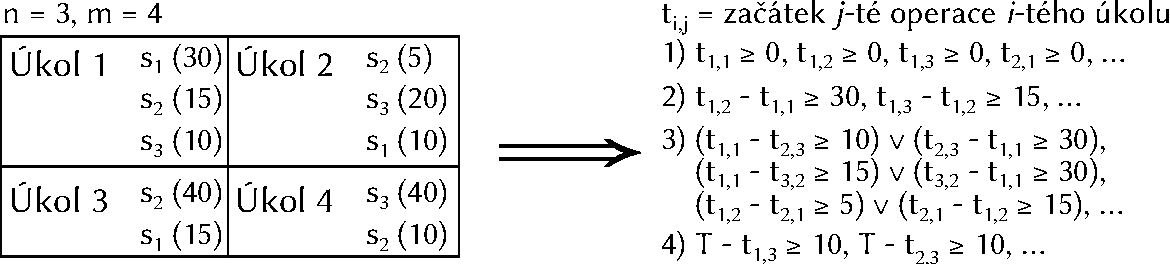
\includegraphics[width=\textwidth]{jobshop.pdf}
	\caption{Příklad převodu plánovacího problému do rozdílových omezení} 
	\label{fig:job}
\end{figure}
\newpage
Cílem této práce je vytvoření STP řešiče pro SMT řešič OpenSMT~\cite{OpenSMT}. Nejprve si přiblížíme některé základní principy z~oblasti SMT řešičů. Následně analyzujeme existující postupy pro řešení STP v~kontextu SMT a~navrhneme podle nich konkrétní algoritmus pro zapojení do OpenSMT. Navržený algoritmus následně implementujeme. Jako součást práce také naši implementaci otestujeme na rozsáhlé sadě problémů a~srovnáme její účinnost s~existujícími SMT řešiči.

\chapter{Analýza}

\section{Fungování SMT řešičů}\label{smt}

Problém splnitelnosti booleovské formule, označovaný též zkratkou SAT, patří k~nejznámějším problémům z~oboru matematické logiky. V~roce 1971 se stal prvním dokazatelně NP-úplným problémem \cite{Cook71} a~v~důsledku toho i~užitečným nástrojem pro teorii složitosti, pomocí něhož lze rozhodovat o~NP-úplnosti dalších problémů.\footnote{Příklady převodů NP-úplných problémů na SAT můžeme nalézt např. v~\cite[kapitola 19]{Mares17}}

V~praktickém použití však SAT naráží na své limitované vyjadřovací schopnosti. Práce s~binárními proměnnými, omezenými pouze na dvě různé hodnoty, může komplikovat převod reálného problému do tvaru booleovské formule. Potřeba užití komplexnějších atomů tak vedla ke zobecnění SAT zvanému \emph{Satisfiability modulo theories} (SMT).

Jak název napovídá, SMT rozšiřuje SAT o~jazyk logických teorií (konkrétně teorií predikátové logiky prvního řádu). máme-li nějakou teorii $t$, pak instancí smt rozumíme formuli jazyka této teorie. jiným pohledem můžeme na instanci smt nahlížet jako na booleovskou formuli, ve které jsme nahradili některé binární proměnné za predikáty obsažené v~$t$. problému vztaženému k~této konkrétní teorii pak říkáme \emph{smt s~ohledem na t}.

jako příklady teorií tradičně řešených v~smt lze uvézt např. teorii lineární aritmetiky (la), teorii neinterpretovaných funkcí s~rovností (euf), či teorii diferenční logiky (dl), kterou se budeme zabývat ve zbytku práce.

vzhledem k~podobnostem mezi sat a~smt není překvapením, že smt řešiče využívají schopností sat řešičů. přechod mezi rozhraním termů teorie a~sat řešičem zpravidla probíhá jedním ze dvou základních způsobů \cite{Nieuwenhuis05}.

první přístup se nazývá \emph{hladový}. hladové smt řešiče operují ve dvou krocích. v~prvním převedou celou vstupní formuli na ekvisplnitelnou booleovskou formuli. druhý krok pak již spočívá jen v~předání této formule existujícímu sat řešiči. pokud bychom tedy pracovali například s~aritmetikou nad osmibitovými čísly, mohli bychom reprezentovat každou proměnnou osmi binárními proměnnými a~aritmetické operace převézt na odpovídající sekvence logických operací.

nespornou výhodou hladových řešičů je možnost použití již existujících metod implementovaných na řešení sat. pro některé teorie se také hladové řešiče ukazují být rychlejší než jejich alternativy. jejich největší problém pak obecně spočívá v~překladu literálů teorie do booleovských formulí. ten musí být zkonstruován samostatně pro každou teorii, a~navíc může v~závislosti na teorii produkovat formule znatelně delší, než byl původní vstup. efektivní převody existují např. pro euf s~omezenou doménou \cite{randal02}, obecně však hladový přístup není příliš rozšířený.

jeho protějškem je takzvaný \emph{líný přístup}. líný přístup se nesnaží měnit strukturu vstupní formule; namísto toho je každý predikát abstrahován pomocí nové binární proměnné. když pak sat řešič rozhodne o~ohodnocení těchto proměnných, oznámí toto rozhodnutí \emph{theory solveru} pro danou teorii. theory solver je schopen určit, zda je dané ohodnocení konzistentní, tzn.~dokáže rozhodnout o~splnitelnosti nějaké konjunkce literálů teorie. sat řešič potom hledá platná ohodnocení, dokud nenajde takové, které theory solver prohlásí za konzistentní.

ve prospěch líných SMT řešičů svědčí fakt, že pro danou teorii často existují dobře známé postupy na ověření konjunkce literálů. Pro LA například můžeme využít metod lineárního programování, theory solver pro DL řeší STP (viz.~\ref{stp}) a~podobně. Mohou však ztrácet efektivitu zejména v~důsledku \emph{slepého prohledávání} \cite{Moura04}, kde hlavní řešič rozhoduje o~hodnotě predikátů, aniž by a~priori věděl o~důsledcích těchto ohodnocení v~rámci teorie, což může vést k~nutnosti vyzkoušet velké množství ohodnocení, než je nalezeno nějaké, které je s~teorií konzistentní.

V~roce 2004 navrhli Gazinger a~kol. nový přístup zvaný \emph{DPLL(T)} \cite{Gazinger04}. DPLL($T$) má koncepčně blíže k~línému vyhodnocování, integruje však těsněji hlavní řešič s~theory solverem. Místo toho, aby využíval theory solveru až po nalezení nějakého ohodnocení, průběžně mu oznamuje dosavadní rozhodnutí a~periodicky se ho ptá na splnitelnost právě dosazené konjunkce. Theory solver pak kromě kontroly splnitelnosti také oznamuje hlavnímu řešiči důsledky této konjunkce. Tím jsme schopni dříve opustit větve rozhodovacího stromu nekonzistentní s~teorií. 

V~jádru tohoto přístupu stojí všeobecný DPLL($X$) engine, využívající DPLL \cite{Davis60} postupu pro SAT řešiče. Tento engine nemusí mít žádné znalosti o~konkrétní teorii. Dosazením theory solveru $Solver_T$ pro danou teorii $T$ za parametr $X$ pak vytvoříme konkrétní instanci DPLL($T$). Hlavní engine komunikuje se $Solver_T$ pomocí následujícího rozhranní \cite{Gazinger04}:

\begin{description}
	\item[Initialize(L: množina literálů).] Inicializuje $Solver_T$ s~$L$ jakožto množinou literálů, které se vyskytují v~problému.
	\item[SetTrue(l: L-literál): množina L-literálů.] Skončí výjimkou, pokud se $l$ ukáže jako nekonzistentní s~dosud zadanými literály teorie. V~opačném případě přidá $l$ do seznamu zadaných literálů a~vrátí množinu L-literálů, které jsou důsledky přidání $l$ do tohoto seznamu.
	\item[IsTrue?(l: L-literál): boolean.] Vrátí \emph{true} právě tehdy, když $l$ je důsledkem seznamu přidaných literálů. \emph{false} tedy vrací, pokud je důsledkem tohoto seznamu $\neg l$, nebo pokud z~něj nevyplývá ani $l$, ani $\neg l$.
	\item[Backtrack(n: přir. číslo).] Odstraní posledních $n$ hodnot ze seznamu zadaných literálů. $n$ nesmí být větší než velikost tohoto seznamu.
	\item[Explain(l: L-literál): množina L-literálů.] Vrátí pokud možno co nejmenší podmnožinu zadaných literálů, z~jejichž konjunkce plyne $l$. Pro $l$ musí platit, že je důsledkem nějaké takové podmnožiny, tedy musí být obsažen v~návratové hodnotě nějakého volání \icode{SetTrue(l')} takového, že $l'$ nebylo zahozeno žádným následným voláním \icode{Backtrack}.
\end{description}

Při použití tohoto rozhranní přitom $Solver_T$ nemusí nic vědět o~implementaci DPLL($X$) enginu. Framework je tedy velice modulární a~snadno rozšiřitelný o~nové teorie. Vyžadujeme pouze, aby byl $Solver_T$ schopný inkrementálně přijímat a~odebírat jednotlivé literály teorie. Tento postup se v~praxi ukazuje jako efektivnější než dostupné alternativy. Většina dnes rozšířených SMT řešičů --- včetně námi používaného OpenSMT2 --- je tedy založena na metodě DPLL($T$).

\section{Rozbor STP}\label{stp}

Jedním ze základních podproblémů vyskytujícím se v~takřka všech plánovacích problémech je takzvaný Simple Temporal Problem (STP). STP poprvé postulovali v~roce 1991 Dechter, Meiri a~Pearl \cite{Dechter91} a~od té doby našel široká využití jak v~informatických oblastech, tak v~oborech od medicíny \cite{Anselma06} po vesmírný let \cite{Fukunaga97}.

Vstupem STP je množina rozdílových omezení, to jest nerovnic tvaru $$x - y \leq c,$$ kde $x$ a~$y$ jsou proměnné a~$c$ je konstanta. V~závislosti na tom, jakou verzi problému řešíme, přitom pracujeme buď s~celočíselnými, nebo s~reálnými hodnotami. Výstupem tohoto problému je pak rozhodnutí, zda existuje ohodnocení proměnných tak, aby byla splněna všechna zadaná omezení. V~rozšíření problému pak můžeme požadovat na výstupu i~nějaké takovéto splnitelné ohodnocení, pokud existuje, případně nalezení pokud možno co nejmenší podmnožiny omezení, která zajišťuje nesplnitelnost problému.

Na první pohled se může zdát pevně daný tvar nerovnic příliš omezující, uvědomme si však, že do této formy můžeme převést několik dalších druhů nerovnic. Nejsnáze zahrneme do problému omezení tvaru $x - y = c$; ty stačí jednoduše nahradit nerovnicemi $x - y \leq c$ a~$x - y \geq c$.

Problematické nejsou ani nerovnice typu $\pm x \leq c$. Pro účely takovýchto omezení si zavedeme novou globální proměnnou $zero$, s~jejíž pomocí převedeme předchozí do tvaru $x - zero \leq c$, respektive $zero - x \leq c$. Pokud pak hledáme splňující ohodnocení proměnných, najdeme takové, kde $zero$ je ohodnoceno nulou. Korektnost tohoto postupu zaručuje následující obecně známé tvrzení.

\begin{tvrz}
	Je-li $\sigma$ splňující ohodnocení nějakého STP a~$\delta$ libovolná konstanta, pak ohodnocení $\pi$ definované pro všechny proměnné $x$ jako $\pi(x) = \sigma(x) + \delta$ je také splňující ohodnocení tohoto STP.
\end{tvrz}
\begin{proof}
	Je-li $\sigma$ splňující ohodnocení, pro libovolné rozdílové omezení $x-y \leq c$ v~problému platí $$\pi(x) - \pi(y) = (\sigma(x) + \delta) - (\sigma(y) + \delta) = \sigma(x) - \sigma(y) \leq c,$$ z~čehož je i~$\pi$ splňující ohodnocení.
\end{proof}

Můžeme do problému zahrnout taktéž omezení tvaru $x - y < c$. Pro celočíselné proměnné lze tuto nerovnici ekvivalentně zapsat jako $x - y \leq c-1$. V~reálné variantě pak nahradíme nerovnici výrazem $x - y \leq c - \delta$, přičemž nenastavujeme okamžitě konkrétní hodnotu $\delta$, ale udržujeme si ji pouze symbolicky a~určujeme její vhodné dosazení až při výpočtu splňujícího ohodnocení. Tento postup je detailněji popsán v~sekci \ref{int_v_real}. Uvědomme si, že pokud jsme schopni vyjádřit ostré nerovnosti, umíme vyjádřit i~negace neostrých nerovností a~naopak.

V~jazyce výrokové logiky pak teorii obsahující výše popsané nerovnice nazveme \emph{teorie diferenční logiky} a~budeme ji značit DL. Celočíselnou variantu této teorie pak budeme značit jako IDL a~reálnou variantu jako RDL. Nahradíme-li pak v~booleovské formuli některé termy těmito nerovnicemi, ověření splnitelnosti takto vzniklé formule je instancí SMT problému s~ohledem na DL.



\section{Převod na grafový problém}\label{graf}

Velkou rozšířenost STP můžeme mimo jiné přisoudit tomu, že jsme schopni ho efektivně řešit. Jelikož se problém skládá výlučně z~lineárních omezení, mohli bychom na první pohled využít metod lineárního programování, jako je například simplexový algoritmus. Tyto metody jsou schopny řešit i~mnohem komplexnější problémy, avšak s~jejich výpočetní silou se pojí znatelně vyšší časová náročnost. Algoritmy specializované na STP se proto už od svého počátku \cite[Kapitola 2]{Dechter91} obracejí jiným směrem, a~to k~formalizmu teorie grafů. Přestože v~průběhu let vzikly různé metody řešení tohoto problému, všechny fungují na základě převedení množiny omezení na takzvaný \emph{omezující graf}.

\begin{definice}[Omezující graf]
	Nechť $\Pi$ je množina rozdílových omezení. Omezujícím grafem této množiny rozumíme hranově ohodnocený orientovaný graf G takový, že vrcholy G tvoří proměnné vyskytující se v~$\Pi$ a~každému omezení $(x-y \leq c) \in \Pi$ odpovídá v~G hrana $\langle x,y\rangle$ s~ohodnocením $c$.
\end{definice}
\begin{pozn}
	Hranu $\langle x,y\rangle$ s~ohodnocením $c$ budeme značit $x \xrightarrow{c} y$. Orientovanou cestu z~$x$ do $y$ se součtem ohodnocení $k$ pak budeme značit $x \xrightarrow{k*} y$.
\end{pozn}

Pro úplnost dodejme, že dvojice proměnných se může vyskytovat v~libovolně mnoha omezeních. Omezující graf je tedy formálně orientovaným multigrafem. Vzhledem k~vzájemné bijekci mezi hranami grafu a~nerovnicemi problému budeme v~průběhu práce volně přecházet mezi oběma reprezentacemi.

Převod do formy grafu je pro řešení problému zásadní. Umožňuje nám totiž formulovat následující klíčové tvrzení.

\begin{tvrz}[Dechter a~kol. \cite{Dechter91}]
	Nechť $\Pi$ je množina rozdílových omezení. Instance STP tvořená touto množinou je splnitelná právě tehdy, když omezující graf $\Pi$ neobsahuje záporné cykly.
\end{tvrz}
\begin{proof}
	Najdeme-li v~omezujícím grafu záporný cyklus obsahující vrchol $x$, sečtením všech nerovnic vyskytujících se v~tomto cyklu dostaneme $x-x \leq c < 0$, z~čehož je jasně problém nesplnitelný. Je-li na druhou stranu problém nesplnitelný, obsahuje $\Pi$ nějakou nerovnici $x - y \leq c$ takovou, že z~$\Pi$ vyplývá $y - x < -c$. Tato implikace znamená, že v~omezujícím grafu existuje cesta $y \xrightarrow{k*} x$ taková, že $k < -c$. Hrana $x \xrightarrow{c} y$ pak společně s~touto cestou tvoří záporný cyklus.
\end{proof}

Hledání splnitelnosti STP jsme tedy schopni převést na hledání záporného cyklu v~grafu. To je problém, který dokážeme efektivně řešit. Využít můžeme např. některý algoritmus na hledání nejkratší cesty, kupříkladu Floydův-Warshallův algoritmus operující v~čase $\Theta(\abs{V}^3)$ nebo Bellmanův-Fordův algoritmus, který má časovou složitost $\Theta(\abs{V}\cdot\abs{E})$.

Tyto algoritmy však trpí pro náš účel zásadním nedostatkem. Jejich použití znamená, že po každém přidání nové hrany do grafu musí znovu proběhnout celé prohledávání. Tento postup není vhodný pro použití v~SMT řešičích, ve kterých je kladen velký důraz na inkrementalitu. V~následující sekci tedy podrobně rozebereme několik postupů pro řešení problémů SMT s~ohledem na DL a~motivujeme výběr námi použitého algoritmu. 

\section{Volba algoritmu}\label{alg}

Jak jsme ukázali v~předchozí sekci, ne všechny algoritmy na rozhodnutí STP jsou dobrou volbou pro použití v~kontextu SMT řešičů. Theory solver pro DPLL($T$) by měl efektivně podporovat dvě zásadní operace --- inkrementální přidávání literálů a~backtracking.

Na rozdíl od základního hladového přístupu, jak byl popsán v~\ref{smt}, v~DPLL($T$) dostává $Solver_T$ informaci o~rozhodnutých ohodnoceních průběžně. Aby byly dříve odhaleny slepé větve v~rozhodovacím stromu, $Solver_T$ je průběžně dotazován na splnitelnost dosud provedených rozhodnutí. Pro zrychlení tohoto procesu je tedy vhodné, aby byl schopen pro výpočet využít výsledků z~předchozích dokončených výpočtů. Algoritmy, které nedokáží takto zakomponovat mezivýpočet podproblému, budou ze své podstaty méně výkonné na postupné sekvenci splnitelných ohodnocení.

Po nalezení nesplnitelného ohodnocení pak neopakuje engine celý výpočet, ale vrací se pouze do nejbližšího stavu, ve kterém bylo ohodnocení ještě splnitelné. Od theory solveru očekáváme, že je schopen efektivně zapomínat přidané literály, vracet se do předchozích stavů a~pokračovat z~nich ve výpočtu. %% FIXME: Better wording?
S~ohledem na tyto požadavky vzniklo několik algoritmů pro řešení SMT s~ohledem na DL. V~této práci se budeme zabývat převážně postupem založeným na vyčerpávající propagaci teorie, který postulovali v~roce 2005 Nieuwenhuis a~Oliveras \cite{Nieuwenhuis05}.

\subsection{DPLL($T$) s~vyčerpávající propagací teorie}

Připomeňme si metodu \icode{SetTrue} uvedenou v~sekci \ref{smt}. Ta slouží k~přidání nového omezení do kontextu řešiče teorie. Řešič může volitelně jako návratovou hodnotu uvést nějakou množinu literálů, které detekoval jako důsledky vzniklé přidáním právě tohoto omezení. Může přitom hlásit např. jen \uv{zjevné} důsledky, popřípadě nemusí vracet vůbec žádné. Pokud jsme je ale schopni nacházet v~rozumém čase, nahlášené důsledky jsou užitečnou informací pro hlavní engine, poněvadž pro něj mohou výrazně zmenšit velikost rozhodovacího stromu.

Varianta DPLL($T$) s~vyčerpávající propagací teorie přidává pro \icode{SetTrue} silnou podmínku; řešič musí vrátit \emph{všechny} literály ze vstupní formule, které jsou důsledky stávajícího ohodnocení. Tento předpoklad značně zjednoduší DPLL($X$) engine a~umožní mu pracovat efektivněji. Stane se z~něj \emph{de~facto} běžný SAT řešič, který se liší pouze minimalistickým rozhranním se $Solver_T$. To má mimo jiné za důsledek, že jsme nyní schopni převézt libovolný SAT řešič na bázi DPLL do DPLL($X$) enginu.

Nevýhoda tohoto přístupu je jasná. Povinnost hledat všechny důsledky teorie může řádově zpomalit operaci \icode{SetTrue} pro řešič teorie. Nicméně se ukázalo, že alespoň v~případě diferenční logiky může tento přístup vést k~rychlé implementaci schopné předčit ostatní alternativy.

\subsection{Návrh řešiče pro diferenční logiku}

$Solver_T$ diferenční logiky využívá principy, se kterými jsme se podrobněji seznámili v~předchozích sekcích. Můžeme například předpokládat, že všechna omezení jsou tvaru $x-y \leq c$ (viz.~\ref{stp}). Využijeme též převodu omezení do tvaru omezujícího grafu, jak bylo uvedeno v~\ref{graf}.

\subsubsection*{Inicializace}
Během inicializace načte řešič vstupní formuli, uloží si všechna rozdílová omezení, která se v~ní vyskytují, a~předá ji DPLL($X$) jako čistě booleovskou formuli. Během tohoto procesu by měl detekovat vztahy mezi literály a~jejich negacemi a~explicitně je poznamenat. Pokud se například na vstupu vyskytnou nerovnice $x-y \leq 1$ a~$y-x \leq -2$, v~oboru celých čísel je jedna negací druhé. Řešič by tak měl abstrahovat tyto výskyty jako $p$ a~$\neg p$ pro booleovskou proměnnou $p$. Ukládá si přitom překladovou tabulku pamatující si pro každou nerovnici abstrahovaný literál, kterému odpovídá. Zároveň s~tím si udržuje pro každou proměnnou seznam všech nerovnic, ve kterých se tato proměnná vyskytuje (účel těchto seznamů je objasněn níže).

\subsubsection*{Ohodnocení literálu}
Jakmile je následně nastavena pravdivostní hodnota některého literálu, převede jej řešič do formy $x-y \leq c$ a~přidá odpovídající hranu do omezujícího grafu. Následně musí objevit všechny důsledky tohoto ohodnocení. Pro jejich nalezení je potřeba zkontrolovat všechny cesty $$x_i \xrightarrow{c_i*} x \xrightarrow{c} y \xrightarrow{c'_j*} y_j$$ a~zjistit, zda nějaké omezení neplyne z~$x_i - y_j \leq (c_i + c + c'_j)$. To budou právě nerovnice tvaru $x_i - y_j \leq c'$, kde $c' \geq c_i + c + c'_j$. 

Abychom prošli všechny tyto cesty, procházející nově přidanou hranou, musíme nejdřív nalézt seznam všech vrcholů $x_i$, ze kterých je dosažitelné $x$, a~seznam všech vrcholů $y_j$, které jsou dosažitelné z~$y$. Omezující graf je tedy reprezentován jako oboustranný seznam sousedů. Potom už můžeme spustit obyčejný algoritmus na hledání nejkratší cesty, kterým získáme všechna vhodná $x_i$ společně s~jejich $c_i$, resp. $y_j$ s~jejich $c'_j$. Autoři pro toto prohledávání doporučují následující postup.

Použijeme běžné prohledávání do hloubky. V~něm si označíme každý vrchol, který jsme navštívili poprvé, společně s~jeho vzdáleností. Navštívíme-li pak již objevený vrchol znovu, pokračujeme v~prohledávání pouze tehdy, když je jeho současná vzdálenost menší než naše uložená vzdálenost. Zároveň si všechny objevené $x_i$ a~$y_j$ ukládáme do dvou odlišných seznamů. Po skončení prohledávání spočteme pro oba seznamy počet všech nerovnic, ve kterých se proměnné v~seznamu vyskytují (tyto nerovnice si pro každou proměnnou pamatujeme z~inicializace).

Vyskytují-li se potom například $x_i$ celkově v~menším počtu proměnných, projdeme pro každé $x_i$ seznam všech nerovnic, ve kterých se vyskytuje, a~zkontrolujeme, zda se nejedná o~důsledek nalezené cesty z~$x_i$ do nějakého $y_j$.

\subsubsection*{Hledání příčin}

Jak víme z~\ref{smt}, řešiče teorie musí implementovat operaci \icode{Explain}, která pro nalezený důsledek vrátí množinu jeho příčin. Tato operace je důležitá pro budování implikačního grafu v~DPLL($X$) a~určení vhodné úrovně backtrackingu při nalezení sporu. Řešič DL popsaný v~\cite{Nieuwenhuis05} tuto operaci provádějí následovně.

Když je do omezujícího grafu přidána $n$-tá hrana, zapamatujeme si k~této hraně její odpovídající $n$. U~nalezených důsledků si pamatujeme $n$ hrany, jejíž přidáním důsledek vznikl. Když pak hledáme vysvětlení hrany $h$ tvaru $x-y \leq c$, spustíme prohledávání z~$x$ do $y$ stejným způsobem jako po přidání hrany. Prohledávání ale pouštíme jen do délky nejvýše $c$ a~jen přes hrany s~číslem vložení nejvýše $n$. Tato omezení zvyšují efektivitu (zmenšujeme prostor k~prohledání) a~zaručují, že nepoužíváme hrany přidané až po důsledku (což by působilo problémy v~implikačním grafu DPLL($X$)). Nalezená cesta tak má délku kratší nebo rovnou $c$ a~sestává se jen z~dříve přidaných hran, z~čehož jasně vidíme, že $h$ je důsledek hran na této cestě.

\subsection{Alternativní řešení}

TODO

\section{Prostředí}

Požadavky na použité prostředí jsou určeny převážně požadavky frameworku OpenSMT, pod nějž tato práce spadá. OpenSMT --- a~tudíž i~tento projekt --- je programován v~jazyce C++, konkrétně ve verzi C++11. Práce byla vyvíjena a~testována na operačním systému s~linuxovým jádrem nad architekturou x64. Jelikož si nejsme vědomi toho, že bychom použili vlastnosti jazyka specifické pro tuto konfiguraci, věříme, že náš kód bude možné bez větších potíží zprovoznit i~na jiných platformách a~operačních systémech.


\chapter{Popis řešení}

\section{Prostředí}

\section{Úpravy referenčního algoritmu}

\section{Datové struktury}

\section{Popis běhu programu}

\section{Srovnání reálné a celočíselné verze}

\chapter{Programátorská dokumentace}

\section{Přidávání literálů}

\section{Hledání důsledků}

\section{Rozhodování o splnitelnosti}

\section{Hledání konfliktů a backtracking}

\section{Nalezení splňujícího ohodnocení}

\chapter{Experimentální měření}

\section{Metodologie}

\section{Výsledky}

\section{Srovnání}


\chapter*{Závěr}
\addcontentsline{toc}{chapter}{Závěr}

V~rámci práce jsme pro OpenSMT vytvořili řešič diferenční logiky nad množinou celých čísel. Seznámili jsme se s~problémem STP, rozebrali jeho vlastnosti a~ukázali jeho transformaci na grafový problém. Zvážili jsme způsoby jeho řešení v~kontextu SMT řešičů a~analyzovali existující algoritmy navržené pro framework DPLL($T$). Popsali jsme metodu vyčerpávající propagace teorie a~její aplikaci pro diferenční logiku.

S~ohledem na tyto poznatky jsme pak implementovali samotný řešič teorie. Naším cílem přitom bylo vytvořit řešič, který bude dobře integrován se zbytkem frameworku a~dosáhne výkonu srovnatelného s~ostatními moderními SMT řešiči. Výsledek naší práce jsme s~těmito řešiči experimentálně srovnali a~ukázali jsme, že se nám podařilo daného cíle dosáhnout --- OpenSMT je srovnatelné či dokonce rychlejší než některé z~nejznámějších SMT řešičů současnosti. Nedosahuje zatím účinnosti těch naprosto nejrychlejších, na jejichž vývoji se soustavně podílí desítky dedikovaných výzkumníků. Věříme ale, že poskytuje dobrý základ, který už v~současné formě nabízí rozumnou alternativu k~současným řešičům a~jehož využitelnost bude růst s~budoucími zlepšeními. 

\subsection*{Možná budoucí rozšíření}

Hlavním úkolem v~nejbližší budoucnosti frameworku je rozšíření našeho řešiče o~podporu problémů nad doménou reálných čísel. S~využitím poznatků uvedených v~sekci~\ref{int_v_real} a~datových struktur již existujících v~OpenSMT máme za to, že by toto rozšíření nemělo být příliš náročné. Většina kódu existujícího v~implementaci celočíselné verze je totiž přenositelná mezi oběma variantami.

Dalším možným směrem budoucího vývoje je práce na zlepšení výkonnosti stávajícího řešiče. Jedním možným směrem této práce by byla analýza implementace použitého algoritmu. Jako příklad uveďme bližší průzkum možnosti použití vícevláknových procesů. Naše zběžné testování tyto přístupy sice zamítlo, ale podrobnější výzkum a~testování by mohly odhalit možnosti ke zrychlení řešiče. Druhou možností pro další výzkum v~tomto směru by pak mohlo být také využití jiných algoritmů v~rámci OpenSMT, ať už by se jednalo o~implementaci již existujících algoritmů, nebo o~vytvoření zcela nových postupů.


%%% Seznam použité literatury
%%% Seznam použité literatury (bibliografie)
%%%
%%% Pro vytváření bibliografie používáme bibTeX. Ten zpracovává
%%% citace v textu (např. makro \cite{...}) a vyhledává k nim literaturu
%%% v souboru literatura.bib.
%%%
%%% Příkaz \bibliographystyle určuje, jakým stylem budou citovány odkazy
%%% v textu. V závorce je název zvoleného souboru .bst. Styly plainnat
%%% a unsrt jsou standardní součástí latexových distribucí. Styl czplainnat
%%% je dodáván s touto šablonou a bibTeX ho hledá v aktuálním adresáři.

\bibliographystyle{czplainnat}    %% Autor (rok) s českými spojkami
% \bibliographystyle{plainnat}    %% Autor (rok) s anglickými spojkami
% \bibliographystyle{unsrt}       %% [číslo]

\renewcommand{\bibname}{Seznam použité literatury}

%%% Vytvoření seznamu literatury. Pozor, pokud jste necitovali ani jednu
%%% položku, seznam se automaticky vynechá.

\bibliography{literatura}

%%% Kdybyste chtěli bibliografii vytvářet ručně (bez bibTeXu), lze to udělat
%%% následovně. V takovém případě se řiďte normou ISO 690 a zvyklostmi v oboru.

% \begin{thebibliography}{99}
%
% \bibitem{lamport94}
%   {\sc Lamport,} Leslie.
%   \emph{\LaTeX: A Document Preparation System}.
%   2. vydání.
%   Massachusetts: Addison Wesley, 1994.
%   ISBN 0-201-52983-1.
%
% \end{thebibliography}


%%% Obrázky v bakalářské práci
%%% (pokud jich je malé množství, obvykle není třeba seznam uvádět)
%%% \listoffigures

%%% Tabulky v bakalářské práci (opět nemusí být nutné uvádět)
%%% U matematických prací může být lepší přemístit seznam tabulek na začátek práce.
%%% \listoftables

%%% Použité zkratky v bakalářské práci (opět nemusí být nutné uvádět)
%%% U matematických prací může být lepší přemístit seznam zkratek na začátek práce.
%%% \chapwithtoc{Seznam použitých zkratek}

%%% Přílohy k bakalářské práci, existují-li. Každá příloha musí být alespoň jednou
%%% odkazována z vlastního textu práce. Přílohy se číslují.
%%%
%%% Do tištěné verze se spíše hodí přílohy, které lze číst a prohlížet (dodatečné
%%% tabulky a grafy, různé textové doplňky, ukázky výstupů z počítačových programů,
%%% apod.). Do elektronické verze se hodí přílohy, které budou spíše používány
%%% v elektronické podobě než čteny (zdrojové kódy programů, datové soubory,
%%% interaktivní grafy apod.). Elektronické přílohy se nahrávají do SISu a lze
%%% je také do práce vložit na CD/DVD. Povolené formáty souborů specifikuje
%%% opatření rektora č. 72/2017.
\appendix
\chapter{Přílohy}

\section{První příloha}

\openright
\end{document}
